% arara: pdflatex
% arara: biber
% arara: pdflatex
% arara: pdflatex

\documentclass[hidelinks, 12pt]{article}%

\usepackage{import}
\usepackage[left=1in, right=1in, top=1in, bottom=1in]{geometry}
\usepackage{hyperref}
\usepackage[tbtags]{amsmath}
\usepackage{amsfonts}
\usepackage{amssymb}
\usepackage[utf8]{inputenc}
\usepackage[T1]{fontenc}
\usepackage{xcolor}
\usepackage{chemformula}
\usepackage[style=ieee,backend=biber]{biblatex}
\usepackage{csvsimple}
\usepackage{siunitx}
\usepackage{float}
\usepackage{graphicx}
\usepackage{listings}

\addbibresource[location=local]{references.bib}

\definecolor{mygreen}{rgb}{0,0.6,0}
\definecolor{mygray}{rgb}{0.5,0.5,0.5}
\definecolor{mymauve}{rgb}{0.58,0,0.82}
\lstset{%
    backgroundcolor=\color{white}, % choose the background color
    breaklines=true, % automatic line breaking only at whitespace
    captionpos=b, % sets the caption-position to bottom
    commentstyle=\color{mygreen}, % comment style
    escapeinside={\%*}{*)}, % if you want to add LaTeX within your code
    keywordstyle=\color{blue}, % keyword style
    stringstyle=\color{mymauve}, % string literal style
    tabsize=2, % Set tabs to be displayed as 2 spaces
    showstringspaces=false, % Don't show string spaces as special characters
    basicstyle=\linespread{1}\footnotesize, % size of fonts used for the code and spacing on the lines (force to 1)
    literate={\ \ }{{}}1, % Convert two spaces to 1 (for soft tab)
    caption={\protect\filename@parse{\lstname}\protect\filename@base\text{.}\protect\filename@ext} % give filename as caption
}

\begin{document}
    \begin{center}
        \vspace*{1cm}
        {\fontsize{300}{50}\selectfont {\bfseries Hello \LaTeX\\}}
        \vspace{3cm}
        {\LARGE An Introduction to the\\
        Typesetting Tool\\}
        \vspace{10cm}
    \end{center}
    \begin{raggedleft}
        {\Large Aaron English\\
            and\\
            Ghassan Arnouk\\
            Date: \today\\}
    \end{raggedleft}
    \thispagestyle{empty}

    \clearpage
    \tableofcontents
    \clearpage
    \section{Motivation}
        \begin{itemize}
            \item High quality documents
            \item Automation
            \item Widely available and extrodinarily flexible
            \item Open-Source (and free)
            \item Enormous and extremely helpful user base
            \item Nearly unlimited skillcap
        \end{itemize}


    \section{Base Packages}
        There are a few base packages that you should always import:
        \begin{enumerate}
            \item import
            \item geometry
            \item hyperref
            \item amsmath
            \item amsfonts
            \item amssymb
            \item inputenc
            \item fontenc
            \item biblatex
            \item float
            \item graphicx
        \end{enumerate}
        
        \begin{lstlisting}[language={[LaTeX]TeX}]
            \usepackage{import}
            \usepackage[left=1in, right=1in, top=1in, bottom=1in]{geometry}
            \usepackage{hyperref}
            \usepackage[tbtags]{amsmath}
            \usepackage{amsfonts}
            \usepackage{amssymb}
            \usepackage[utf8]{inputenc}
            \usepackage[T1]{fontenc}
            \usepackage[style=ieee,backend=biber]{biblatex}
            \usepackage{float}
            \usepackage{graphicx}
        \end{lstlisting}

    \section{Sections...}
        \subsection{...and subsections...}
            \subsubsection{...and subsubsections...}

    \section{Equations}
        How about some equations?
        \begin{align}
            \delta &= - \frac{B^{2}}{180,000} + \frac{B}{173} + 0.5\nonumber\\
            &= - \frac{533^{2}}{180,000} + \frac{533}{173} + 0.5 \nonumber\\
            &= 2.0 \nonumber
        \end{align}
        
        Or even a matrix 1
        \begin{equation*}
            A = 
            \begin{bmatrix}
                -\alpha-\beta & 2 & \frac{1}{c}\\
                -4i & \sqrt{5-\alpha} & -6\\
                c & \beta & 9 + i
            \end{bmatrix}
        \end{equation*}

        Calculus!
        \begin{align}
            \frac{\text{d}x}{\text{d}t} &= \sigma (y-x)\\
            \frac{\text{d}y}{\text{d}t} &= x(\rho -z)-y\\
            \frac{\text{d}z}{\text{d}t} &= xy-\beta z
        \end{align}

    \clearpage
    \section{Figures}
        You can add lovely figures, and then reference them like this "As stated in Figure \ref{fig:test}".
        It's even a hyperlink \textit{*click* *click*}

        \begin{figure}[htbp]
            \begin{centering}
                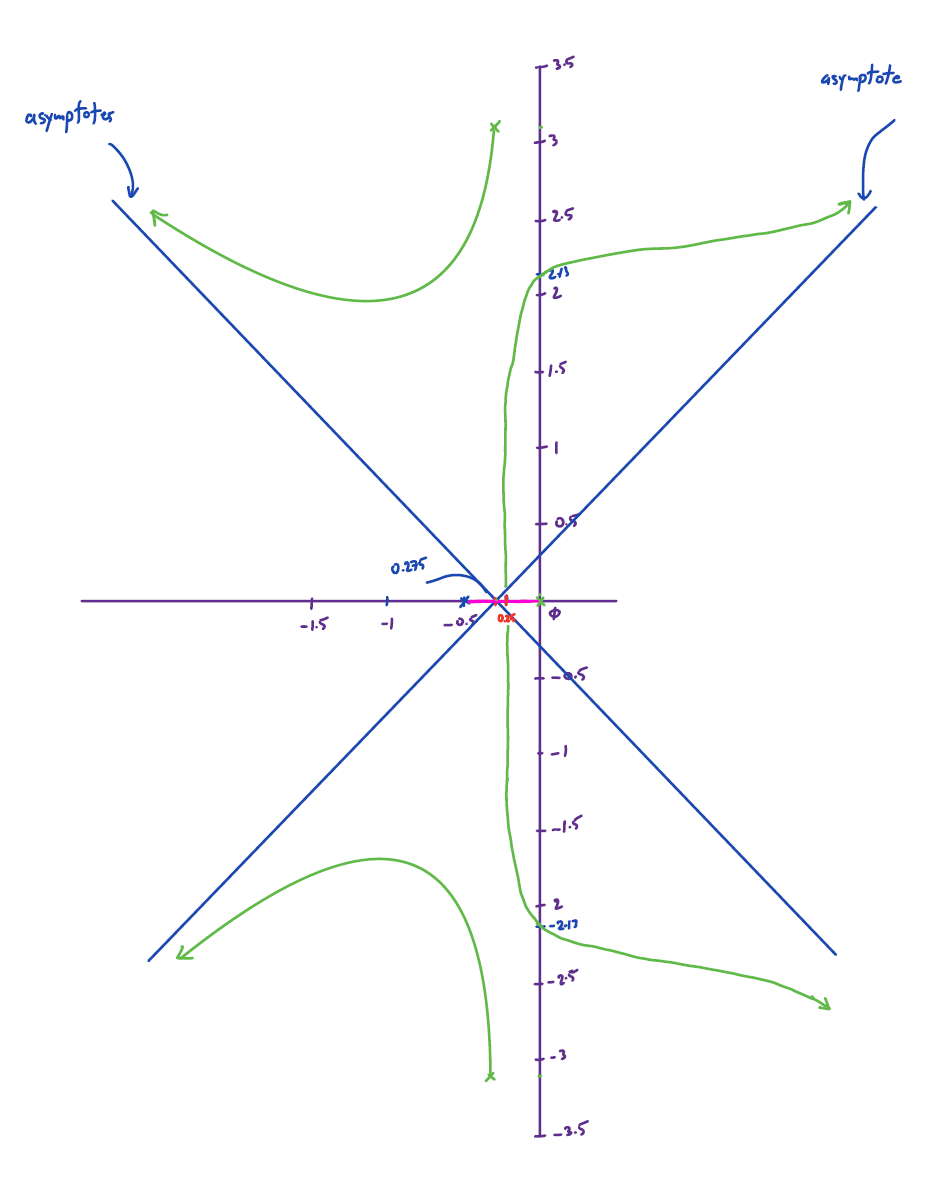
\includegraphics[width=0.5\textwidth]{images/rootLocus.png}
                \caption{A test figure}
                \label{fig:test}
            \end{centering}
        \end{figure}

    \clearpage
    \section{Tables}
        What are tables like?
        Like this!
		\begin{table}[H]
			\centering
			\caption{Table of specified parameters and achieved values}
            \vspace{0.2cm}
			\begin{tabular}{c|c|c|c}
				 & \bfseries Target & \bfseries Values & \bfseries Results
				\csvreader[head to column names]{data/TargetsAndVals.csv}{}
				{\\\hline\csvcoli & \csvcolii & \csvcoliii & \csvcoliv }
			\end{tabular}
			\label{Table:Parameters}
		\end{table}

    \section{Additional Helpful Packages}
    \begin{itemize}
        \item siunitx
            I strongly recommend using the siunitx package for formatting all units.
            \\\si{\hertz}
            \\\SIrange{100}{200}{\nano\meter}
            \\\SI{100}{\kilo\gram}
            \\Convenient!
        \item xcolor
            for {\color{red}colourful} {\color{blue}text}!

        \item listings

            \begin{lstlisting}[language=python]
                def string2bits(s=''):
                    return [bin(ord(x))[2:].zfill(8) for x in s]

                def bits2string(b=None):
                    return ''.join([chr(int(x, 2)) for x in b])

                s = 'Hello, World!'
                b = string2bits(s)
                s2 = bits2string(b)

                print 'String:'
                print s

                print '\nList of Bits:'
                for x in b:
                    print x

                print '\nString:'
                print s2
            \end{lstlisting}

        \item chemformula
            A chemistry equation!
            \begin{equation}
               \ch{
                    ^{2}H + ^{2}H -> ^{3}He + n^{0}
                }
                \label{eqt:nucEnerReleased}
            \end{equation}
    \end{itemize}


    \section{Bibliography}
        \subsection{Writing the .bib File}
            \begin{lstlisting}[language={[LaTeX]TeX}]
                @incollection{ref:01,
                    author = {Berger, M.J. and Hubbell, J.H. and Seltzer, S.M. and Chang, J. and Coursey, J.S. and Sukumar, R. and Zucker, D.S. and Olsen, K.},
                    title = {XCOM: Photon Cross Sections Database},
                    publisher = {NIST, PLM, Radiation Physics Division},
                    year = {2010},
                    booktitle = {NIST Standard Reference Database 8 (XGAM)},
                    chapter = {Copper},
                    url = {https://physics.nist.gov/cgi-bin/Xcom/xcom3_1},
                }
            \end{lstlisting}
        \subsection{Using the References}
            Here I am making a statement that should be backed up with a reference placed here -> \cite{ref:01}
            Now it will show up in the bibliography and the reference above will link to it and be 
            correctly numbered. For Free!
        
    \clearpage
    \printbibliography[heading=bibintoc]
\end{document}
